\documentclass[tikz,border=12pt]{standalone}
\usepackage{amsmath}
\usetikzlibrary{arrows.meta,positioning}
\definecolor{pink}{HTML}{F72585}\definecolor{blue}{HTML}{4DABF7}
\definecolor{green}{HTML}{51CF66}\definecolor{ink}{HTML}{343A40}\definecolor{soft}{HTML}{F1F3F5}
\begin{document}
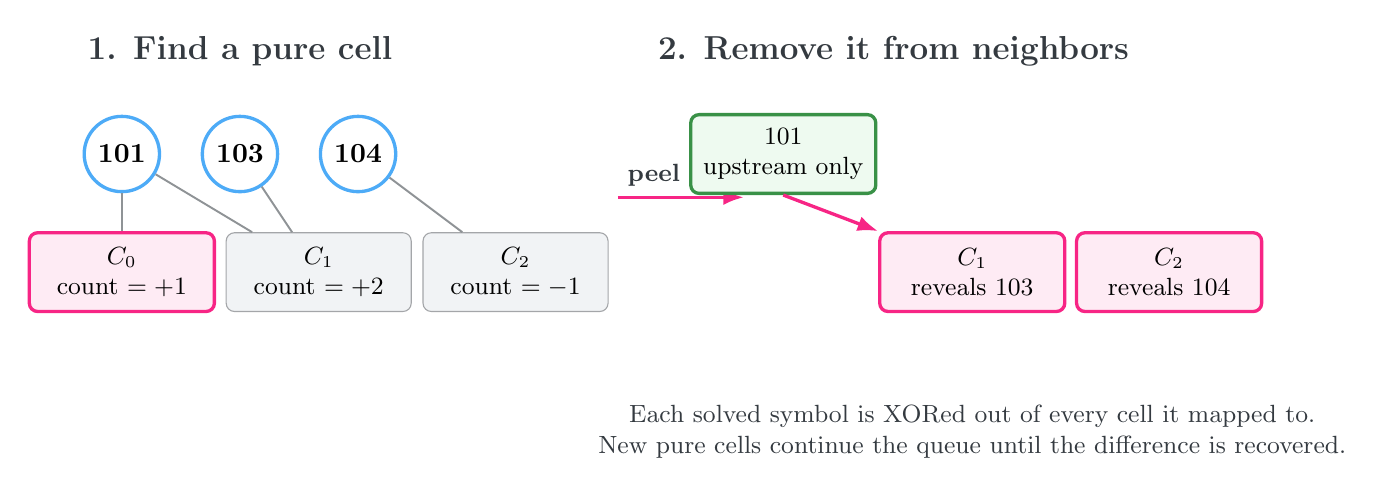
\begin{tikzpicture}[
 symbol/.style={circle,draw=blue,fill=white,very thick,minimum size=9mm,font=\bfseries},
 cell/.style={rounded corners=3pt,draw=ink!45,fill=soft,minimum width=2.35cm,minimum height=1cm,align=center,font=\small},
 pure/.style={cell,draw=pink,fill=pink!9,very thick},
 solved/.style={cell,draw=green!70!black,fill=green!10,very thick},
 edge/.style={ink!55,line width=.7pt},peel/.style={-{Latex[length=2.6mm]},pink,very thick},
 title/.style={font=\bfseries\large,text=ink}]
 \node[title] at (0,2.35) {1. Find a pure cell};
 \node[symbol] (s101) at (-1.5,1.05) {101}; \node[symbol] (s103) at (0,1.05) {103};
 \node[symbol] (s104) at (1.5,1.05) {104};
 \node[pure] (c0) at (-1.5,-.45) {$C_0$\\count $=+1$};
 \node[cell] (c1) at (1,-.45) {$C_1$\\count $=+2$};
 \node[cell] (c2) at (3.5,-.45) {$C_2$\\count $=-1$};
 \draw[edge] (s101)--(c0); \draw[edge] (s101)--(c1); \draw[edge] (s103)--(c1); \draw[edge] (s104)--(c2);
 \draw[peel] (4.8,.5) -- node[above,text=ink,font=\small\bfseries]{peel 101} (6.4,.5);
 \begin{scope}[xshift=8.3cm]
  \node[title] at (0,2.35) {2. Remove it from neighbors};
  \node[solved] (r101) at (-1.4,1.05) {$101$\\upstream only};
  \node[pure] (r103) at (1,-.45) {$C_1$\\reveals $103$};
  \node[pure] (r104) at (3.5,-.45) {$C_2$\\reveals $104$};
  \draw[peel] (r101.south) -- (r103.north west);
  \node[below=1.05cm of r103,align=center,font=\small,text=ink]
   {Each solved symbol is XORed out of every cell it mapped to.\\New pure cells continue the queue until the difference is recovered.};
 \end{scope}
\end{tikzpicture}
\end{document}
